\section{Introduction}

Recently, Linux containers have drawn a significant amount of attention because they are lightweight, portable, and repeatable.
Linux containers are generally more lightweight than virtual machine (VM) clusters, because the containers share the kernel with the host operating system (OS), even though they maintain separate execution environments.
They are generally portable because the process execution environments are archived into tar files,
so whenever one attempts to run a container, the exact same file systems are restored from the archives
even when totally different data centers are used.
This means that containers can provide repeatable and portable execution environments.
%
For the same reasons, Linux containers are attractive for web services as well,
and it is expected that web services consisting of container clusters would be
capable of being migrated easily for a variety of purposes. For example disaster recovery,
cost performance improvements, legal compliance, and shortening the geographical distance to customers
are the main concerns for web service providers in e-commerce, gaming, Financial technology(Fintech) and Internet of Things(IoT) field.
%

Kubernetes\cite{K8s2017}, which is one of the popular container cluster management systems, 
enables easy deployment of container clusters.
Since Kubernetes hides the differences in the base environments, users can easily deploy a web service on different 
cloud providers or on on-premise data centers, without adjusting the container cluster configurations to the new environment. 
This allows a user to easily migrate a web service consisting of a container cluster even to the other side of the world. 
A user starts the container cluster in the new location, route the traffic there, 
then stop the old container cluster at his or her convenience.
This is a typical web service migration scenario.

However, this scenario only works when the user migrates a container cluster among major cloud providers including Google Cloud Platform (GCP), 
Amazon Web Services (AWS), and Microsoft Azure.
The Kubernetes does not provide generic ways to route the traffic from the internet into container cluster and is 
heavily dependent on external load balancers that are set up on the fly by cloud providers through their application protocol interfaces (APIs).
%
These external load balancers distribute incoming traffic to every server that hosts containers.
The traffic is then distributed again to destination containers using iptables destination 
network address translation (DNAT)\cite{MartinA.Brown2017,Marmol2015} rules in a round-robin manner. 
The problem happens in the environment with a load balancer that is not supported by the Kubernetes, 
e.g. in an on-premise data center with a bare metal load balancer. 
In such environments, the user needs to manually configure 
the static route for inbound traffic in an ad-hoc manner. 
Since the Kubernetes fails to provide a uniform environment from a container cluster viewpoint,
migrating container clusters among the different environments will always be a burden.

In order to solve this problem by eliminating the dependency on external load balancers,
we have proposed a containerized software load balancer that is run by Kubernetes as  
a part of web service container clusters in the previous work\cite{takahashi2018portable}.
It enabled a user to deploy a web service in different environments without modification easily 
because the web service itself includes load balancers.

We containerized Linux kernel's Internet Protocol Virtual Server (IPVS)\cite{Zhang2000} 
Layer 4 load balancer using an existing Kubernetes ingress\cite{K8sIngress2017} framework, as a proof of concept.
%
%
We also proved that our approach does not significantly deteriorate the performance,
by comparing the performance of our proposed load balancer with those of
iptables DNAT load balancer and the Nginx Layer 7 load balancing.
%
The results indicated that the proposed load balancer could improve the portability of container clusters without performance degradation compared with the existing load balancer.

However, in our previous work, we did not discuss the redundancy of such load balancers.
Routing traffic to one of the load balancers while keeping redundancy in the container environment is a complex issue
because standard Layer 2 redundancy protocols, e.g., Virtual Router Redundancy Protocol(VRRP)\cite{hinden2004virtual}
or OSPF\cite{moy1997ospf}, which uses multicast, cannot be used in many cases.
Furthermore, providing uniform methods independent of the infrastructures such as various cloud environments and the on-premise data center is much more difficult.

In this paper, we extend the previous work and propose a software load balancer with Equal Cost Multi-Path(ECMP)\cite{thaler2000multipath} redundancy for container cluster environment where a cloud load balancer compatible with Kubernetes does not exist.
We containerize an open source BGP software, exabgp\cite{exa-networks_2018}, and launch it with containerized Linux kernels IPVS load balancer as a single pod using Kubernetes.
We set up a redundant load balancer cluster using such pods and evaluate its functionality.
We also measure the preliminary performance of such a load balancer cluster.

The contributions of this paper are as follows:
1) We propose a portable software load balancer with ECMP redundancy for container cluster environments without cloud load balancers.
2) We implement such a load balancer using existing Open Source Software(OSS).
2) We demonstrate the basic functionality, i.e., redundancy and scalability of such s load balancers.
Proving that it is possible to design and implement a scalable web service using OSS tools will benefit users who want to migrate their web service to outside of the major cloud providers.

The rest of the paper is organized as follows.
Section \ref{Related Work} highlights work that deals specifically with container cluster migration,
software load balancer containerization, and load balancer related tools within the context of the container technology.
Section \ref{Proposed Architecture} will explain existing architecture problems and propose our solutions.
In Section \ref{Implementation}, experimental conditions and the parameters
that we considered to be important in our experiment will be described in detail.
Then, we will show our experimental results and discuss the obtained performance characteristics in Section~\ref{Evaluation}, which is followed by a summary of our work in Section~\ref{Conclusions}.

\section{Related Work}\label{Related Work}

This section highlights related work, especially that dealing with container cluster migration, 
software load balancer containerization, load balancer tools within the context of the container technology and scalable load balancer in the cloud providers.

\paragraph{\bf Container cluster migration:}

Kubernetes developers are trying to add federation\cite{K8sFederation2017} capability for handling situations 
where multiple Kubernetes clusters\footnote{The {\em Kubernetes cluster} refers to a server cluster 
controlled by the Kubernetes container management system, in this paper.} 
are deployed on multiple cloud providers or on-premise data centers, 
and are managed via the Kubernetes federation API server (federation-apiserver). 
However, how each Kubernetes cluster is run on different types of cloud providers
and/or on-premise data centers, especially when the load balancers of such environments are not supported by Kubernetes, 
seems beyond the scope of that project. 
The main scope of this paper is to make Kubernetes usable in environments 
without supported load balancers by providing a containerized software load balancer.

\paragraph{\bf Software load balancer containerization:}
As far as load balancer containerization is concerned, the following related work has been identified:
Nginx-ingress\cite{Pleshakov2016,NginxInc2016} utilizes the ingress\cite{K8sIngress2017} capability of Kubernetes, 
to implement a containerized Nginx proxy as a load balancer. Nginx itself is famous as a high-performance web server program
that also has the functionality of a Layer-7 load balancer. Nginx is capable of handling Transport Layer Security(TLS) encryption, 
as well as Uniform Resource Identifier(URI) based switching. However, the flip side of Nginx is that it is much slower than Layer-4 switching.
We compared the performance between Nginx as a load balancer and our proposed load balancer in this paper.
%
Meanwhile, the kube-keepalived-vip\cite{Prashanth2016} project is trying to use Linux kernel's IPVS\cite{Zhang2000} 
load balancer capabilities by containerizing the keepalived\cite{ACassen2016}.
The kernel IPVS function is set up in the host OS's net namespaces and is shared among multiple web services,
as if it is part of the Kubernetes cluster infrastructure.
Our approach differs in that the IPVS rules are set up in container's net namespaces 
and function as a part of the web service container cluster itself.
The load balancers are configurable one by one, and are  movable with the cluster once the migration is needed.
The kube-keepalived-vip's approach lacks flexibility and portability whereas ours provide them.
%
The swarm mode of the Docker\cite{DockerCoreEngineering2016,DockerInc2017} also uses IPVS for internal load balancing,
but it is also considered as part of Docker swarm infrastructure, 
and thus lacks the portability that our proposal aims to provide.

\paragraph{\bf Load balancer tools in the container context:}
There are several other projects where efforts have been made to utilize IPVS in the context of container environment.
For example, GORB\cite{Sibiryov2015} and clusterf\cite{Aaltodoc:http://urn.fi/URN:NBN:fi:aalto-201611025433} are daemons 
that setup IPVS rules in the kernel inside the Docker container. 
They utilize running container information stored in key-value storages
like Core OS etcd\cite{CoreOSEtcd} and HashiCorp's Consul\cite{HashiCorpConsul}. 
Although these were usable to implement a containerized load balancer in our proposal, we did not use them, 
since Kubernetes ingress framework already provided the methods to retrieve running container information through standard API.

\paragraph{\bf Cloud load balancers:}

As far as the cloud load balancers are concerned, two articles have been identified.
Google's maglev\cite{eisenbud2016maglev} is a software load balancer used in Google Cloud Platform(GCP)\cite{Voellm2013}.
Maglev uses modern technologies including per flow ECMP and kernel bypass for userspace packet processing.
Maglev serves as the GCP's load balancer that is used by the Kubernetes.
Maglev can be solely used in GCP, and the users need open source software load balancer that is runnable even in on-premise data centers.
Microsoft's Ananta\cite{patel2013ananta} is another software load balancer implementation using ECMP and windows network stack.
Ananta can be solely used in Microsoft's Azure cloud infrastructure\cite{patel2013ananta}.
The proposed load balancer by the author is different in that it is aimed to be used in every cloud provider and on-premise data centers.

\section{Proposed Architecture}\label{Proposed Architecture}

Here we discuss a generall overview of the proposed load balancer architectures.

%\subsection{A containerized Load balancer}

\subsection{Problems of Kubernetes Cluster}

\begin{figure}
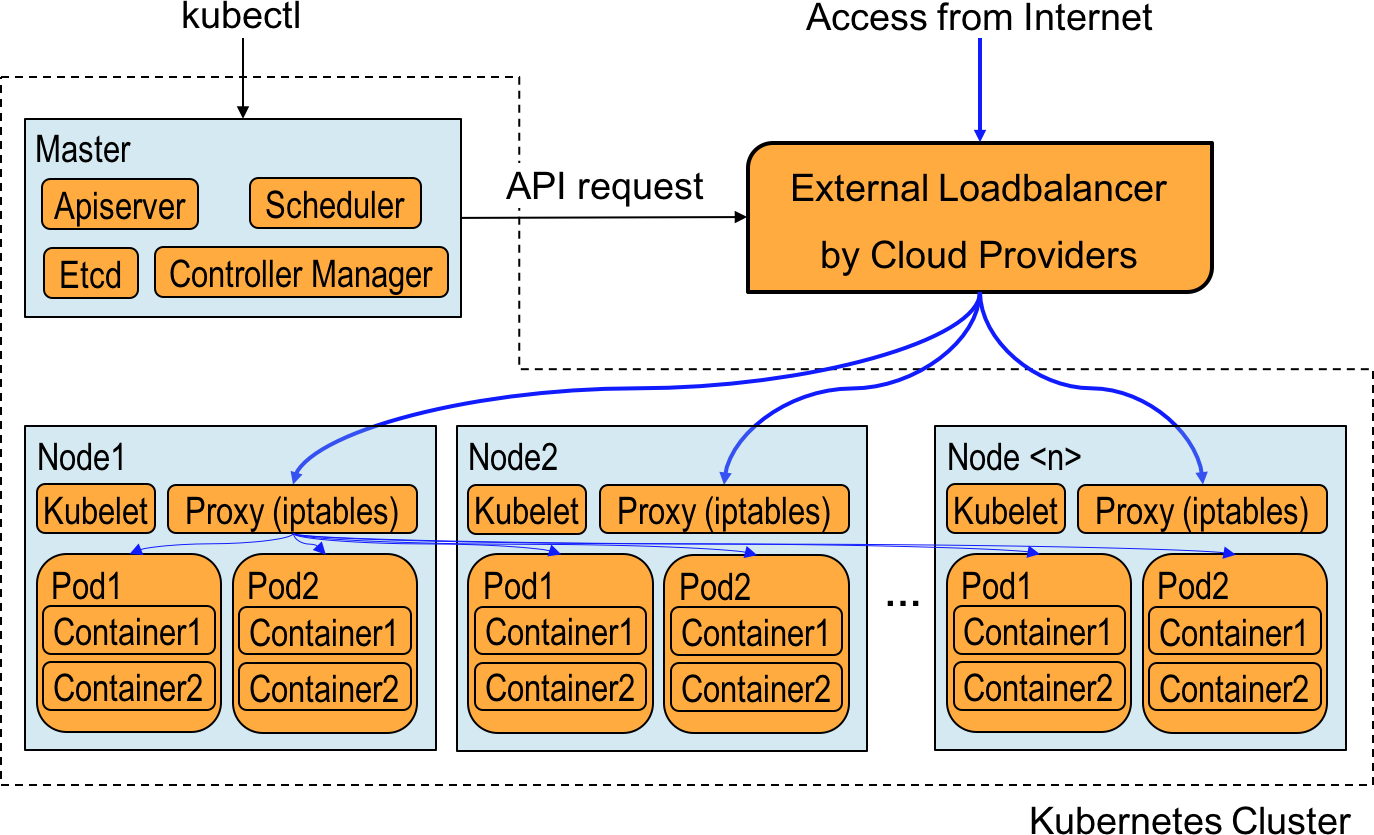
\includegraphics[width=\columnwidth]{Figs/K8sConventional}
\caption{Conventional architecture of a Kubernetes cluster.}
\label{fig:K8sConventional}
\end{figure}

Problems commonly occur when the Kubernetes container management system is used outside of recommended cloud providers(such as GCP or AWS).
Figure~\ref{fig:K8sConventional} shows an exemplified Kubernetes cluster.
A Kubernetes cluster typically consists of a master and nodes. They can be physical servers or VMs.
On the master, daemons that control the Kubernetes cluster are typically deployed. 
These daemons include, apiserver, scheduler, controller-manager and etcd. 
On the nodes, the kubelet daemon will run {\it pods}, depending the PodSpec information obtained from the apiserver on the master.
A {\em pod} is a group of containers that share same net namespace and cgroups, 
and is the basic execution unit in a Kubernetes cluster.

When a service is created, the master will schedule where to run {\em pods} and kubelets on the nodes will launch them accordingly.
At the same time, the masters will send out requests to cloud provider API endpoints, asking them to set up external load balancers.
The proxy daemon on the nodes will also setup iptables DNAT\cite{MartinA.Brown2017} rules. 
The Internet traffic will then be evenly distributed by the external load balancer to nodes, 
after which it will be distributed again by the DNAT rules on the nodes to the designated {\em pods}. 
The returning packets will follow the exact same route as the incoming ones.

This architecture has the followings problems: 
1) Having external load balancers whose APIs are supported by the Kubernetes daemons is a prerequisite. 
There are numerous load balancers which is not supported by the Kubernetes.
These include the bare metal load balancers for on-premise data centers.  
In such cases, a user could manually setup the routing table on the gateway so that the traffic would be routed to one of the nodes.
Then the traffic would be distributed by the DNAT rules on the node to the designated {\em pods}.
However, this approach would require complicated network configuration and significantly degrade the portability of container clusters.
2) Distributing the traffic twice, first on the external load balancers and second on each node, 
complicates the administration of packet routing. 
Imagine a situation in which the DNAT table on one of the nodes malfunctions.
In such a case, only occasional timeouts would be observed, which would make it very difficult to find out which node was malfunctioning.   

In short, 1) Kubernetes can be used only in limited environments where the external load balancers are supported, 
and 2) the routes incoming traffic follow are very complex.
%
To address these problems, we propose a containerized software load balancer with ECMP redundancy for container cluster environment without a cloud load balancer.

\subsection{Proposed architecture: a potable load balancer}

\begin{figure}
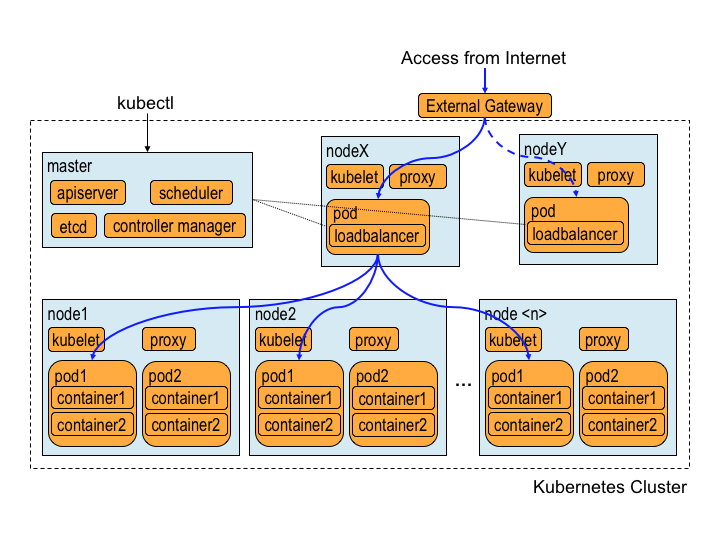
\includegraphics[width=\columnwidth]{Figs/K8sProposed}
\caption{Kubernetes cluster with proposed load balancer.}
\label{fig:K8sProposed}
\end{figure}

Figure~\ref{fig:K8sProposed} shows the proposed  Kubernetes cluster architecture, 
which has the following characteristics:
1) Each load balancer itself is run as a {\em pod} by Kubernetes. 
2) Load balancer configurations are dynamically updated based on information about running {\em pods}.
%%3) There exist multiple load balancers for redundancy. 
The proposed load balancer can resolve the conventional architecture problems, as follows:
Since the load balancer itself is containerized, load balancer can run in any environment including on-premise data centers, 
even without external load balancers that is supported by Kubernetes.
The incoming traffic is directly distributed to designated {\em pods} by the load balancer. 
It makes the administration, e.g. finding malfunctions, easier.

We designed the proposed load balancer using three components, IPVS, keepalived, and a controller. 
These components are placed in a Docker container image.
The IPVS is a Layer-4 load balancer capability, which is included in the Linux kernel 2.6.0 released in 2003 or later, 
to distribute incoming Transmission Control Protocol(TCP) traffic to 
{\em real servers}\footnote{The term, {\em real servers} refers to worker servers that will respond to incoming traffic, 
in the original literature\cite{Zhang2000}. We will also use this term in the similar way.}\cite{Zhang2000}. 
For example, IPVS distributes incoming Hypertext Transfer Protocol(HTTP) traffic destined for a single destination IP address, 
to multiple HTTP servers(e.g. Apache HTTP or nginx) running on multiple nodes in order to improve the performance of web services.
Keepalived is a management program that performs health checking for {\em real servers}
and manage IPVS balancing rules in the kernel accordingly.
It is often used together with IPVS to facilitate ease of use.
The controller is a daemon that periodically monitors the {\em pod} information on the master, 
and performs various actions when such information changes.
Kubernetes provides ingress controller framework as the Go Language(Golang) package to implement such controllers. 
We have implemented a controller program that will feed {\em pod} state changes to keepalived 
using this framework. 

\subsection{Proposed architecture: load balancer redundancy}

\paragraph{\bf Overlay network}

In order to discuss redundancy, the knowledge of the overlay network is essential.
We briefly explain an abstract concept of overlay network that is common to existing overlay network including flannel\cite{coreos_2018} and calico\cite{project_calico}.

\begin{figure}[tb]
\begin{center}
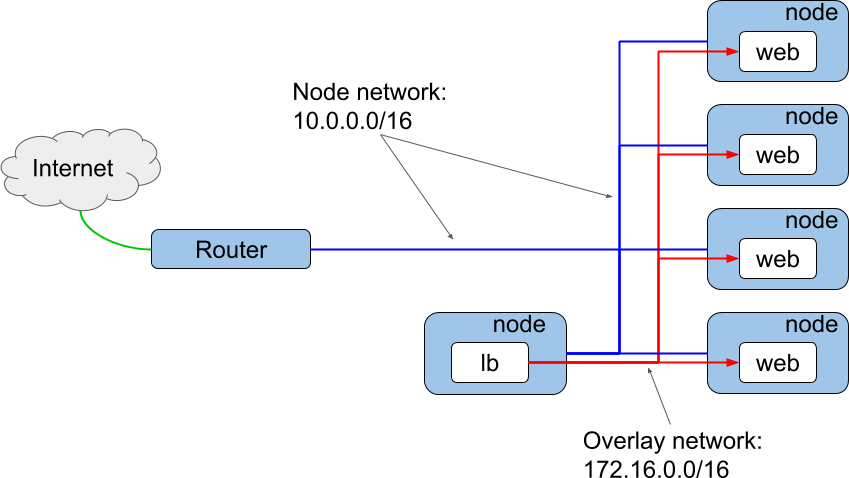
\includegraphics[width=\columnwidth]{Figs/overlay.png}
\end{center}
\caption{
  The network architecture of an exemplified container cluster system.
  A load balancer(lb) pod(the white box with "lb") and web pods are running on nodes(the blue boxes).
  The traffic from the internet are forwarded to the lb pod by the upstream router using the node network,
  and the distributed to web pods using the overlay network.
}
\label{fig:overlay}
\end{figure}

Fig.~\ref{fig:overlay} shows schematic diagram of network architecture of a container cluster system. 
An overlay network consists of appropriate routing tables on nodes, and optionally of tunneling setup using ipip or vxlan.
The overlay network is the network for containers to communicate with each other. 
The node network is the network for nodes to communicate with each other. 
The upstream router usually belongs to the node network.
When the ipvs container in the Fig.~\ref{fig:overlay} communicates with the other nodes, 
the nodes can properly route the packets because they have the routes to 172.16.0.0/16 in their routing tables, 
which is a part of overlay network setups.
When a container communicates with the upstream router that has no knowledge of the overlay network, the souce IP address must be translated by Source Network Address Translation(SNAT) rules on each node.

\paragraph{\bf Redundancy with ECMP}

The ECMP is a functionality a router may support, where the router has multiple next hops with equal cost(priority) to a destination, and generally distribute the traffic depending on the hash of the flow 5 tuples(source IP, destination IP, source port, destination port, protocol).
The multiple next hops and their cost are often populated using the Border Gateway Protocol(BGP) protocol.

\begin{figure}[tb]
\begin{center}
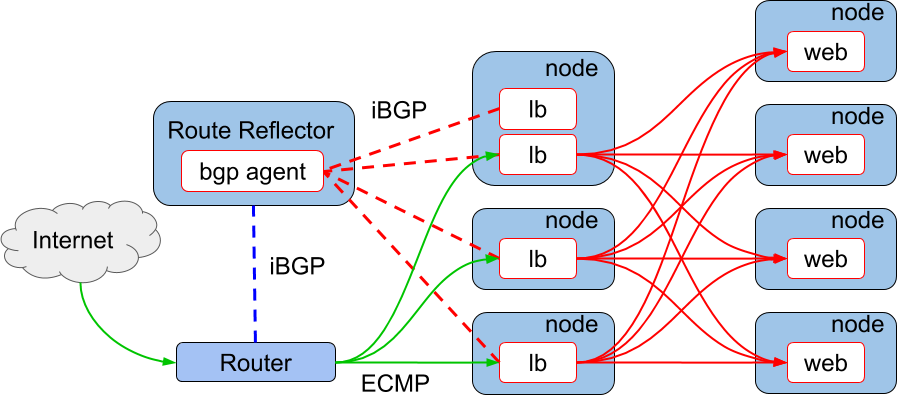
\includegraphics[width=\columnwidth]{Figs/ecmp.png}
\end{center}
\caption{
  The proposed architecture of load balancer redundancy.
  The traffic from the internet is distributed by the upstream router to multiple of lb pods using hash-based ECMP and then distributed by the lb pods to web pods using Linux kernel's ipvs.
  The ECMP routing table on the upstream router is populated using iBGP.
}
\label{fig:ecmp}
\end{figure}

Fig.~\ref{fig:ecmp} shows our proposed redundancy architecture with ECMP for software load balancer containers.
%
We propose to use a node with the knowledge of overlay network as a Route Reflector, in other to alleviate the following problems.
%
1) If we were to setup BGP peering directly between a load balancer container and the router, the IP address of the container should be translated using SNAT rules by a node, since the router has no knowledge of the overlay network and cannot send out returning packet correctly.
However, if we use SNAT, the router usually cannot set up multiple BGP session from a single node even if there are multiple load balancers on that node, because the router only sees the node IP address as the peer.
This problem poses limitation that a single node can accommodate only one load balancer at most and hence we may not be able to utilize underlying node performance fully.
%
2) Also, if we were to setup BGP peering directly between a load balancer container and the router, the router should support so-called dynamic peering(or dynamic neighbor) functions.
When the dynamic peering is supported, one can do without specifying every possible IP address for peers by specifying the IP address range.
This function is essential because one cannot predict IP addresses of the load balancer containers before he launches them.
Even if the router supports such functions, the administrator of the upstream router may not like accepting dynamic peering from wide range of random IP addresses for security reasons.

Since we can use standard Linux boxes for route reflectors we can configure them as we like, e.g., we can make them so that multiple BGP sessions from a single node can be established, and BGP sessions with load balancers are set up dynamically.
The upstream router does not need to accept BGP session from containers with random IP addresses, but only from the Router Reflector with well known fixed IP address.
Although not shown in the Fig.~\ref{fig:ecmp}, we could also place another Route Reflector for redundancy.

The notable benefit of the ECMP setup is the fact that it is scalable.
All load balancer that claims as the next hop is active, i.e., the traffic is forwarded to them depending on the flow tuple.
The traffic is distributed by the upstream router. Hence the overall throughput is determined by the router after all.
But still, if a software load balancer is capable of handling 1 Gbps equivalent of traffic and the upstream router is capable of handling 10 Gbps, it is worthwhile launching 10 of the software load balancer containers to fill up maximum throughput of the upstream router.

\paragraph{\bf Redundancy with VRRP}

\begin{figure}[tb]
\begin{center}
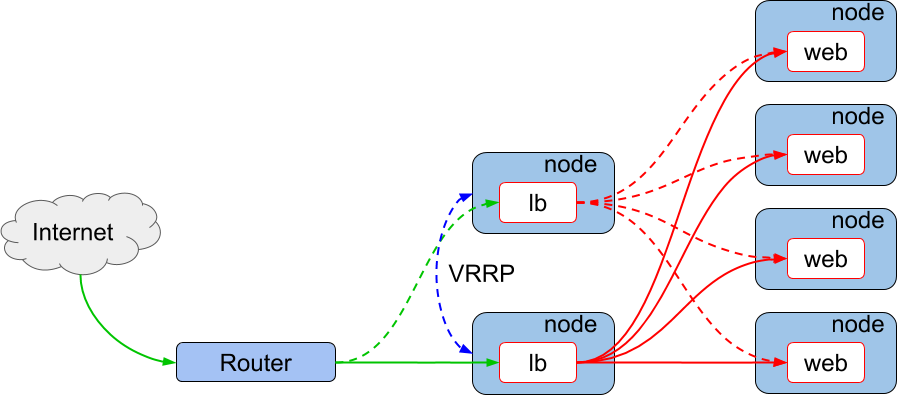
\includegraphics[width=\columnwidth]{Figs/vrrp.png}
\end{center}
\caption{
  An alternative redundant load balancer architecture using.
  The traffic from the internet is forwarded by the upstream router to a active lb node and then distributed by the lb pods to web pods using Linux kernel's ipvs.
  The active lb pod is selected using VRRP protocol.
}
\label{fig:vrrp}
\end{figure}

Fig.~\ref{fig:vrrp} shows an alternative redundancy setup using the VRRP protocol.
In the case of VRRP, the load balancer container needs to run in the node net namespace for the following two reasons.
1) When failover occurs, the new master sends gratuitous Adress Resolution Packets(ARP) packets to update the ARP cache of the upstream router and Forwarding Data Base(FDB) of layer 2 swicthes during the transition.
Such gratuitous ARP packets should consist of the virtual IP address shared by the load balancers and the MAC address of the node where the new master load balancer is running.
Programs that send out gratuitous ARP with node MAC address should be in the node net namespace.
%
2) Furthermore, the active load balancer sends out periodic advertisement using UDP multicast packet to inform existence of itself.
The receiving load balancer in backup state stays calm unless the VRRP advertisement stops for a specified duration of time.
The UDP multicast is often unsupported in overlay network used by container cluster environment, and hence the load balancer needs to be able to use the node net namespace.
%
VRRP programs also support unicast advertisement by specifying IP addresses of peer load balancers when it starts.
However, container cluster management system randomly assign IP addresses of containers when it launches them.
Therefore the unicast mode is not feasible in container cluster environment.
%
Running containers in the node net namespace lose the whole point of containerization, i.e., they share the node network without separation.
This requires the users' additional efforts to avoid conflict in VRRP configuration.

The other drawback compared with the ECMP case is that the redundancy of VRRP is provided in Active-Backup manner.
This means that a single software load balancer limits the overall performance of the entire container cluster.
Therefore we believe the ECMP redundancy is better than VRRP in our use cases.

\section{Implementation}\label{Implementation}

Here we discuss the implementation of expermintal system to prove the concept of our proposed load balancers with ECMP redundancy in detail.

\subsection{Experimental system architecture}

\begin{figure}[tb]
\begin{center}
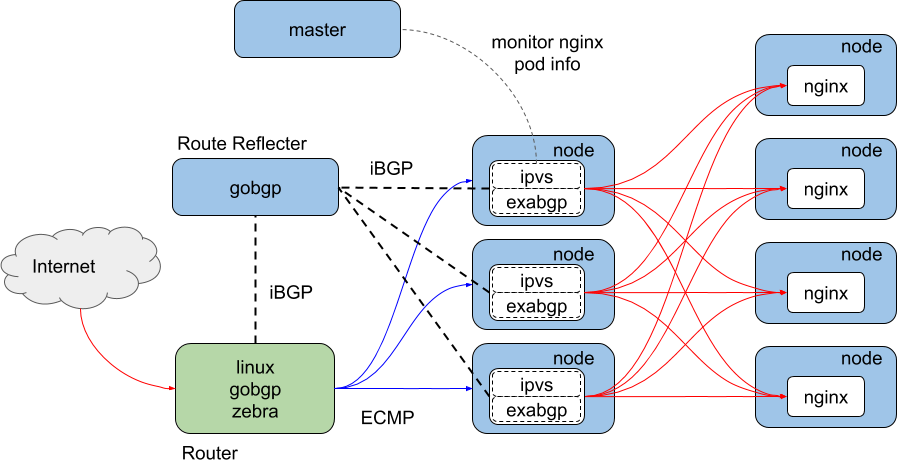
\includegraphics[width=\columnwidth]{Figs/poc.png}
\end{center}
\caption{
  An experimental container cluster with porposed redundant software balancers.
  The master and nodes are configured as Kubernetes's master and nodes on top of conventional linux boxes, respectively.
  The route reflector and the upstream router are also conventional linux boxes.
}
\label{fig:poc}
\end{figure}

Fig.~\ref{fig:poc} shows the shcematic diagram of proof of concept container cluster system with our porposed redundant software load balancers.
All the nodes and route reflector are configured using Debian 9.5 with self compiled linux-4.16.8 kernel.  
The upstream router also used conventional linux box using the same OS as the nodes and route reflector.
For the linux kernel to support hash based ECMP routing table we needed to use kernel version 4.12 or later.
We also needed to enable kernel config option CONFIG\_IP\_ROUTE\_MULTIPATH\cite{ip-sysctl}.
In the actual production environment, proprietary hardware with the highest throughput is often deployed, but we could test some of the required advanced functions by using a Linux box.

The load balancer pods consist of an exabgp container and an ipvs container.
The IPVS container is responsible for distributing the traffic toward a service IP to web(nginx) server pods.
The IPVS container monitors the availability of web server pods and manages the load balancing rule appropriately.
The exabgp container is responsible for advertising the route toward a service IP, to the route reflector.
The route reflector aggregates the routing information advertised by load balancer pods and advertise them to the upstream router.

The exabgp is used in the load balancer pods because of the simplicity in setting as static route advertiser.
On the other hand, gobgp is used in the router and the route reflector, because exabgp did not seem to support add-path\cite{walton2016advertisement} needed for multi-path advertisement and Forwarding Information Base(FIB) manipulation\cite{exa-networks_2018}.
The gobgp supports the add-path, and the FIB manupilation through zebra\cite{osrg_gobgp_zebra}.
The configurations for the router is summarised in \ref{appendix:router_config}.

The route reflector also used a linux box with gobgp and overlay network setup[..... add more info].
The configurations for the route reflector is summarised in \ref{appendix:route_reflector_config}.

\subsection{IPVS container}

\begin{figure}
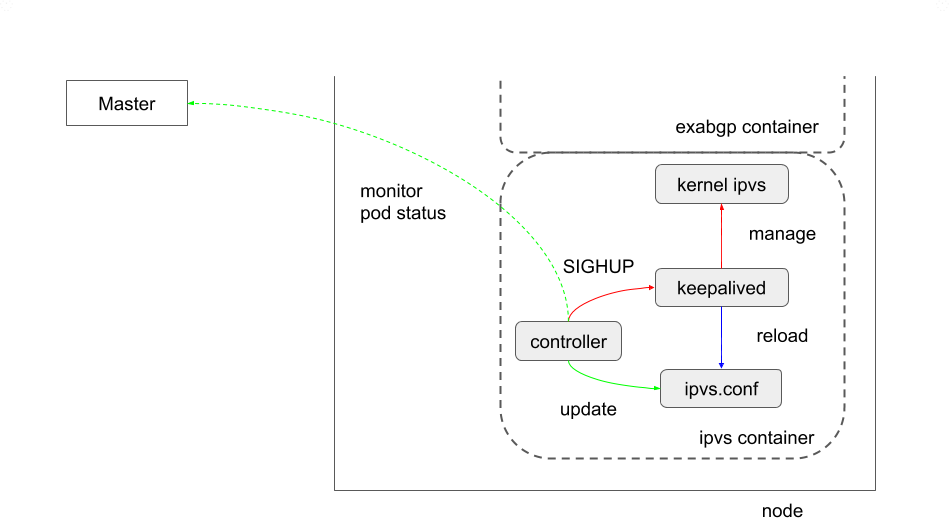
\includegraphics[width=\columnwidth]{Figs/ipvs-ingress-schem}
\caption{Implementation of IPVS container.}
\label{fig:ipvs-ingress-schem}
\end{figure}

The proposed load balancer needs to dynamically reconfigure the IPVS balancing rules whenever {\em pods} are created/deleted. 
Fig.~\ref{fig:ipvs-ingress-schem} is a schematic diagram of IPVS container to show the dynamic reconfiguration of the IPVS rules.
Two daemon programs, controller and keepalived, run in the container inside the LB2 pod are illustrated.
The keepalived manages Linux kernel's IPVS rules depending on the ipvs.conf configuration file.
It is also capable of health-checking the liveliness of {\em real server}, 
which is represented as a combination of the IP addresses and port numbers of the target {\em pods}. 
If the health check to a {\em real server} fails, keepalived will remove that {\em real server} from the IPVS rules.

The controller monitors information concerning the running {\em pods} of a service 
in the Kubernetes cluster by consulting the apiserver running in the master.
Whenever {\em pods} are created or deleted, the controller will automatically regenerate an appropriate ipvs.conf 
and issue SIGHUP to keepalived.
Then, keepalived will reload the ipvs.conf and modify the kernel's IPVS rules accordingly.
The actual controller\cite{ktaka_ccmp_2017_826894} is implemented using the Kubernetes ingress controller\cite{K8sIngress2017} framework. 
By importing existing Golang package, \enquote{k8s.io/ingress /core/pkg/ingress}, we could simplify the implementation, e.g. 
120 lines of code.  

Keepalived and the controller are placed in the docker image of IPVS container.
The IPVS is the kernel function and namespace seperation for container has already been supported in the recent Linux kernel. 

%In this way, the IPVS's balancing rules inside Linux kernel are maintained so that it can distribute the incoming traffic only to the living pods.

Configurations for capabilities were needed when deploying the IPVS container: adding the CAP\_SYS\_MODULE capability 
to the container to allow the kernel to load required kernel modules inside a container, 
and adding CAP\_NET\_ADMIN capability to the container to allow keepalived to manipulate the kernel's IPVS rules. 
For the former case, we also needed to mount the \enquote{/lib/module} of the node's file system on the container's file system.

\subsection{BGP software container}

\begin{figure}
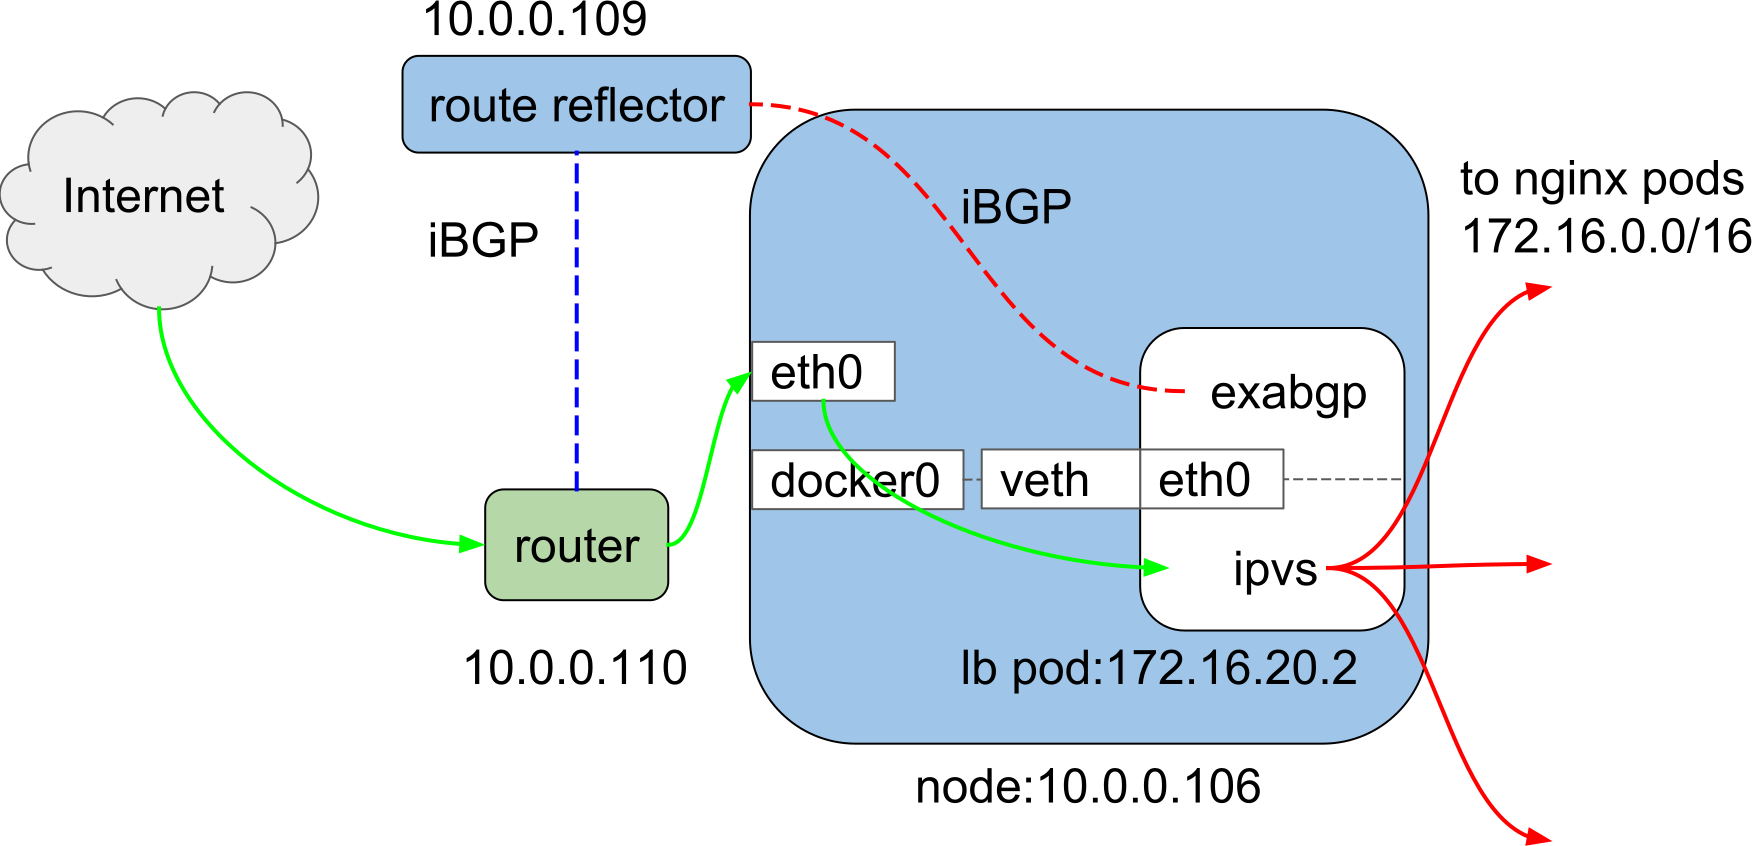
\includegraphics[width=\columnwidth]{Figs/exabgp}
\caption{Implementation of exabgp container.}
\label{fig:exabgp}
\end{figure}

Fig.~\ref{fig:exabgp} shows a schematic diagram of a BGP container. We used exabgp as the BGP advertiser as mentioned earlier.
Table~\ref{table:exabgp} summarises some key settings required for the exabgp container.
The node IP address, 10.0.0.106 is used as next-hop for the service IP range 10.1.1.0/24 in BGP annoucement since the upstream router has no knowledge of assigned to a exabgp container. 
In oder to route the packets toward the service IPs to a container, a routing rule to the dev docker0 is created in the node net namespace for the route to properly accept the packets and route them to the container.
A routing rule to accept the packets as local is also required in the container net namespace. 
A configuration of exabgp is shown in \ref{appendix:exabgp_config}.

\begin{table}[tb]% 
\begin{center}
\begin{tabular}{l}
\hline
\textbf{BGP announcement:}\\
\hspace*{5mm} route 10.1.1.0/24 next-hop 10.0.0.106 \\
\textbf{Routing in node net namespace:}\\
\hspace*{5mm} ip netns exec node ip route replace 10.1.1.0/24 dev docker0 \\
\textbf{Accept as local:}\\
\hspace*{5mm} ip route add local 10.1.1.0/24 dev eth0 \\
\hline
\end{tabular}
\halflineskip

\caption{
  The required settings in exabgp container.
  The node IP address, 10.0.0.106 is used as next-hop for the service IP range 10.1.1.0/24 in BGP annoucement.
  In oder to route the packets toward the service IPs to a container, a routing rule to the dev docker0 is created in the node net namespace.
  A routing rule to accept the packets as local is also required. 
}
\label{table:exabgp}

\end{center}
\end{table}

\section{Evaluation}\label{Evaluation}

We examined the basic performance of the our proposed load balancer container and the basic function of the ECMP redundancy.
As for the performance, we measured throught of the load balancer container and found that it was at least as good as existing software load balancer using Linux. The portability of the load balancer is obvious as we made it runnable as the container usig Kubernetes.  
The ECMP redundancy is examined by watching routing table updates on the router when the new load balancer is add or removed. 
We also demonstrate two diffrent service with different number of load balancers can share the group of nodes.

\subsection{Load balancer performance}

Fig.~\ref{fig:ipvs-iptables-nginx} shows the throughput of the proposed IPVS load balancer in a container.
The throughput is measured by sending out http requests from a benchmark program called wrk\cite{Glozer2016} on a benchmark host towards the load balancer pod and counting the number of responses the benchmark host recieved in a second.
Also shown are the nginx as the load balancer and the iptables DNAT as the Round Robin load balancer as references. 
As we increased the number of the web server conianers from 1 to around 14 the peformance of the IPVS pod increased almost linierly and after which it saturated. 
The increase is considered as the evidence of the benefit of placing a load balancer in front of web servers and let the web servers share the load.
The saturated peformance level indicated the maximum peformance of the cluster consisting of one load balancer and multiple web server pods.
In this particular experiment it turned out the band width of the 1 Gbps bandwidth of network used in the expriment\cite{takahashi2018portable}.
While nginx did not show any benefit as the load balancer, the peformance of the IPVS load balancer container showed equivalent performance level as the iptables DNAT load balancing in the node net namespace. 
This means that our proposed portable load balancer container is as good as the uncontainerized iptables' load balancing to the extent of the 1 Gbps network speed. 

\begin{figure}
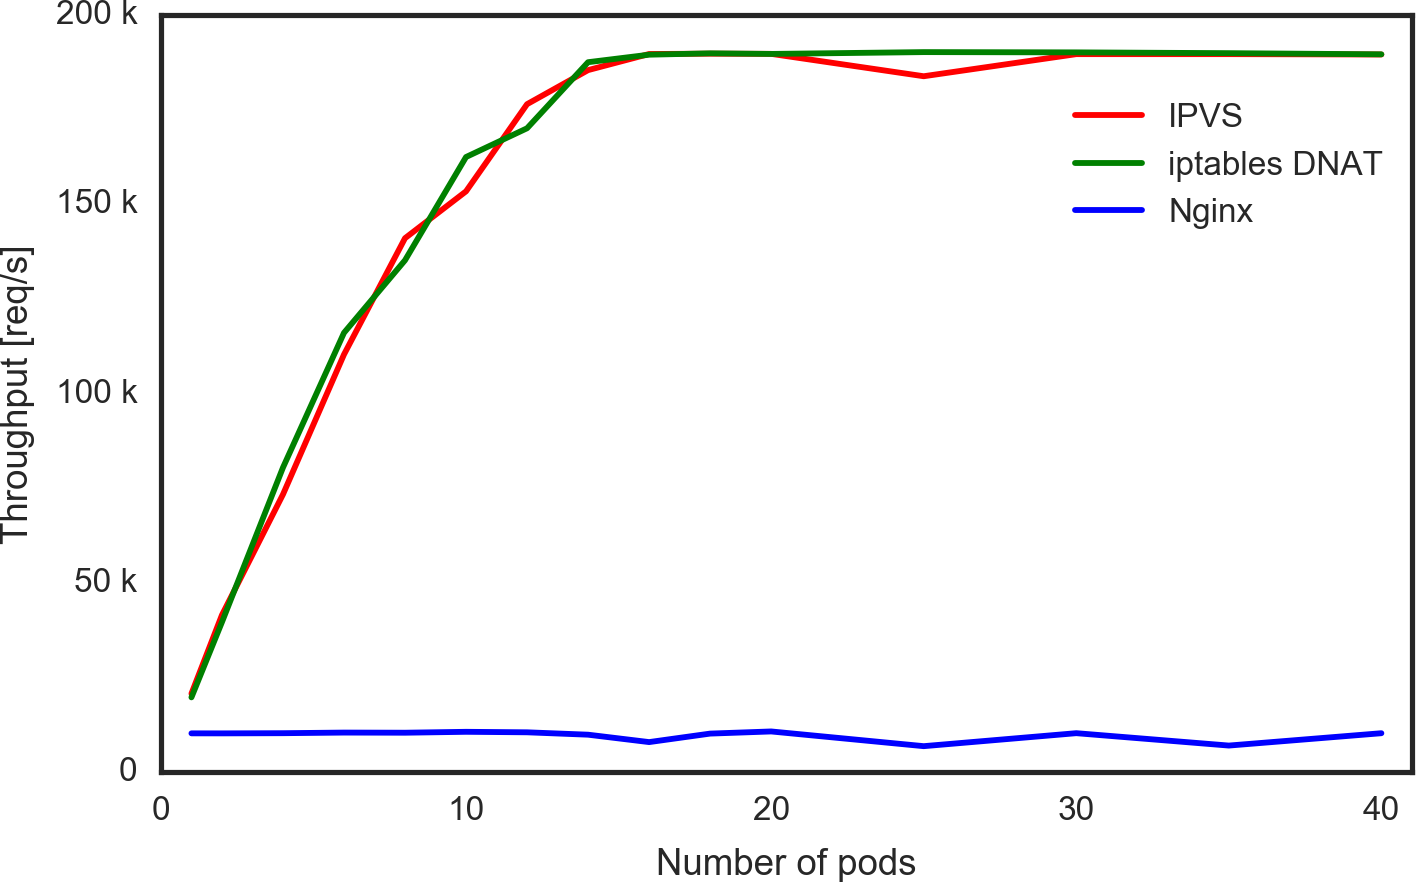
\includegraphics[width=\columnwidth]{Figs/ipvs-iptables-nginx}
\caption{Performance of the load balancer container.}
\label{fig:ipvs-iptables-nginx}
\end{figure}

\subsection{ECMP route population}

The ECMP redundancy is expected to give us the load balancer redundancy and scalability since all the load balancer containers act as active.
In this subsection we evaluated behavior of the ECMP routing table updates, which is equivalnt realizing redundancy. 

The Listing~\ref{single_lb} shows the routing table entry on the router when single load balancer pod exists.
From this line we can understands that packets toward 10.1.1.0/24 are forwarded to 10.0.0.106 where the load balancer pod is running.
It also shows that this routing rule is controled by zebra.

\begin{lstlisting}[language=bash,caption=Routing table entry with single load balancer pod.,label=single_lb]
10.1.1.0/24 via 10.0.0.106 dev eth0 proto zebra metric 20
\end{lstlisting}

When the number of the load balancer pods is incrased to three, we can see the routing table entry as the Listing~\ref{three_lb}.
We have three next hops towards 10.1.1.0/24 each of which beeing the node where the load balancer pods are running.
The weights of the three nexthops are all 1.   

\begin{lstlisting}[language=bash,caption=Routing table entry with three load balancer pods.,label=three_lb]
10.1.1.0/24 proto zebra metric 20
        nexthop via 10.0.0.105  dev eth0 weight 1
        nexthop via 10.0.0.106  dev eth0 weight 1
        nexthop via 10.0.0.107  dev eth0 weight 1
\end{lstlisting}

%{\bf The ECMP is functioning .... packets are arriving for both load balancers.
%W need evidence of pakets arriving all pods.. }

The Listing~\ref{double_services} shows the case where we started new service with two load balancer pods with service addresses in 10.1.2.0/24 range.
We could accomodate two diffrent services toward different IP addresses, one with three load balancers and the other with two load balancers on a group of nodes(10.0.0,105,10.0.0,106,10.0.0,107). 
Again, the population of the routing entry was almost instant as we started the load balancers for the second service.


\begin{lstlisting}[language=bash,caption=Routing table entry with additional service with two load balancer pods started.,label=double_services]
10.1.1.0/24 proto zebra metric 20
        nexthop via 10.0.0.107  dev eth0 weight 1
        nexthop via 10.0.0.105  dev eth0 weight 1
        nexthop via 10.0.0.106  dev eth0 weight 1
10.1.2.0/24 proto zebra metric 20
        nexthop via 10.0.0.107  dev eth0 weight 1
        nexthop via 10.0.0.106  dev eth0 weight 1
\end{lstlisting}



\section{Conclusions}\label{Conclusions}


In this paper, we proposed a portable load balancer for the Kubernetes cluster systems 
that is aimed at facilitating migration of container clusters for web services.
We implemented a containerized software load balancer that is run by Kubernetes as a part of container cluster, 
using Linux kernel's IPVS, as a proof of concept.
We also proposed ECMP redundacy architecture for our portable load balancers. 
In order to discuss the feasibility of the proposed portable load balancer with ECMP redundancy, we built 
a system with multiple web severs and  the load balancer container using  Kubernetes cluster management system and conducted performance measurements.
Our experimental results indicate that the IPVS based load balancer in container improves the portability of 
the Kubernetes cluster system while it shows the similar performance levels as the existing iptables DNAT based load balancer.
We also implemented ECMP redundancy using group of load balancer pods and examined basic functionality. 
Our experimental system consists of standard Linux boxes and OSSs, which was good for testing out latest technology for our proposed ECMP redundancy architecture. 
We could success fullybuild the experimental system that function as our proposed achitecture should.
  

We also clarified that choosing the right operating modes of overlay networks is important for the performance of load balancers. 
For example, in the case of flannel, only the vxlan and udp backend operation modes could be used 
in the cloud environment, and the udp backend significantly degraded their performance.
Furthermore, we also learned that the distribution of packet processing among multiple CPUs was very important
to obtain the maximum performance levels from load balancers.

In this paper we porposed portable load balancer architecture with ECMP redundancy.
To realize the portability we containerized IPVS and made it work in the Kubernetes.
We implemented experimental system to prove that such arhichtecture works using standard Linux boxes and OSS.



In this paper, we proposed a portable software load balancer that has the following features, 1) runnable as a Linux container, 2) redundancy with ECMP technique, for the container cluster systems.

Our load balancer aims at facilitating migration of container clusters for web services.
We implemented a containerized software load balancer that is run by Kubernetes as a part of container cluster,
using Linux kernel's IPVS.

To discuss the feasibility of the proposed load balancer, we built
a Kubernetes cluster system and conducted performance measurements.
Our experimental results indicate that the IPVS based load balancer in container improves the portability of
the container cluster while it shows the similar performance levels as the existing iptables DNAT based load balancer.

We also started to the implementation of a novel software load balancer using recently introduced Linux kernel's XDP infrastructure.
While it is in a preliminary stage of the development, essential functions and design issues have been already clarified.
They will be presented at the time of the presentation.

\section{Future work}\label{Future work}

BGP peering with the Route Reflector is one way of providing a uniform environment for web service container clusters.
While providing a software load balancer that can be controlled through API is another way.
For the former, corporation by the cloud provider so that users can use BGP peering with the upstream router is essential.
In case such a corporation cannot be made, the latter is also worth investigating.


